%
%6-test-suite-and-drivers.tex
%
%  LaTeX source file for section 6 Test Suite and Drivers for the Conceptual Clustering lab module of the TAILS project.
%
\section{Test Suite and Drivers}

\subsection{Using the default setting}
Click \emph{Use Default} in the first interface and then follow these five steps. 
\begin{enumerate}[1)]
\item Choose \emph{circle,large,green}, enter \emph{8} in the \emph{Add Multiple} button and click it.
\item Choose \emph{circle,large,red}, enter \emph{2} in the \emph{Add Multiple} button and click it.
\item Choose \emph{square,small,green}, enter \emph{4} in the \emph{Add Multiple} button and click it.
\item Choose \emph{square,small,blue}, enter \emph{7} in the \emph{Add Multiple} button and click it.
\item Choose \emph{circle,large,blue} and click the \emph{Add} button.
\end{enumerate}

Or you may choose \emph{Use Default} in the first interface and then load the following text to the text box at the bottom of the second interface.\\
circle,large,green!circle,large,green!circle,large,green!circle,large,green!circle,large,green!\\circle,large,green!circle,large,green!circle,large,green!circle,large,red!circle,large,red!\\square,small,green!square,small,green!square,small,green!square,small,green!square,small,blue!\\square,small,blue!square,small,blue!square,small,blue!square,small,blue!square,small,blue!\\square,small,blue!circle,large,blue!

Either way, a classification tree shown in Figure\ref{Fig:testsuite} will be generated. We can see that the last object, a blue circle is grouped to the class consists of two red circles and eight green circles. The remaining objects, including four green squares and seven blue squares are in the same class. This classification tree corresponds to the example on Page 5. 
\begin{figure}[h!]
    \centering
    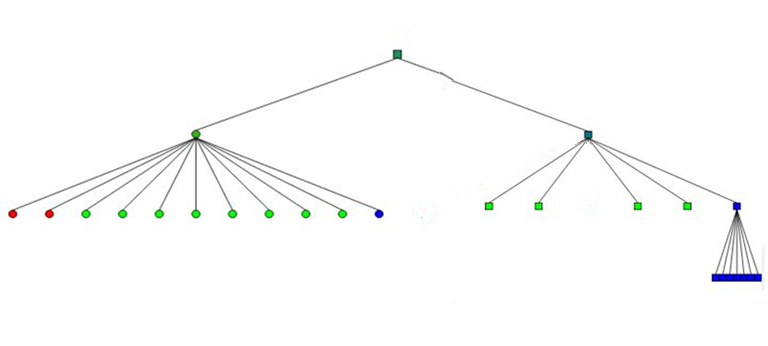
\includegraphics[width=300pt]{../images/testsuite.jpg}
    \caption{}
    \label{Fig:testsuite}
	\end{figure}